\documentclass[../main.tex]{subfiles}
\graphicspath{{\subfix{../../images/}}}

\begin{document}

\subsection{IP addresses}
\label{2:sec:ip}

IP stands for the Internet Protocol, and IP addresses are like street addresses; in the sense that they \emph{represent locations on a network}. This allows for data to be transmitted between devices. There are 2 main types, IPv4 and IPv6 addresses.

\begin{figure}[h]
    \centering
    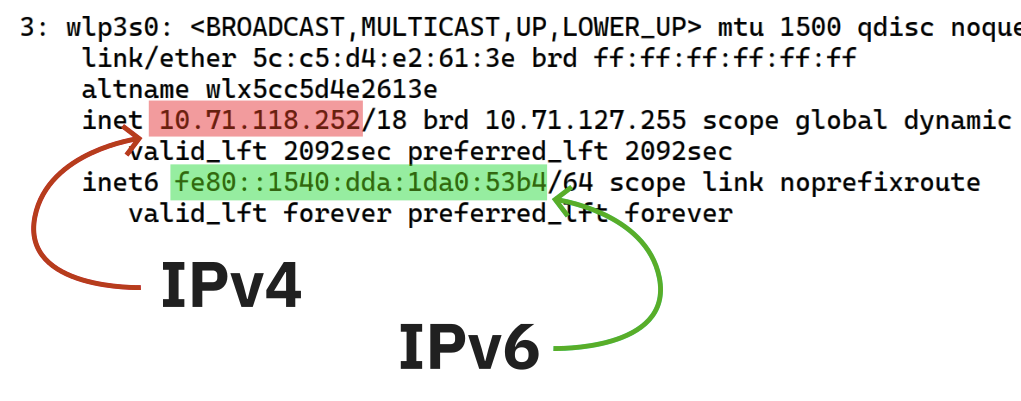
\includegraphics[width=0.7\textwidth]{ip_addresses}
    \caption{Output from the Linux {\ccmono ip} utility, showing IPv4 and V6 addresses}
\end{figure}

\paragraph{IPv4 Addresses}

Are \textbf{32-bit values} represented as 4 3-digit numbers with dots between them, like {\ccmono 192.168.0.1} with each value ranging between 0-255. There are 2 tyes of IP addresses, \emph{Public} and \emph{Private} IP addresses.

\begin{figure}[h]
    \centering
    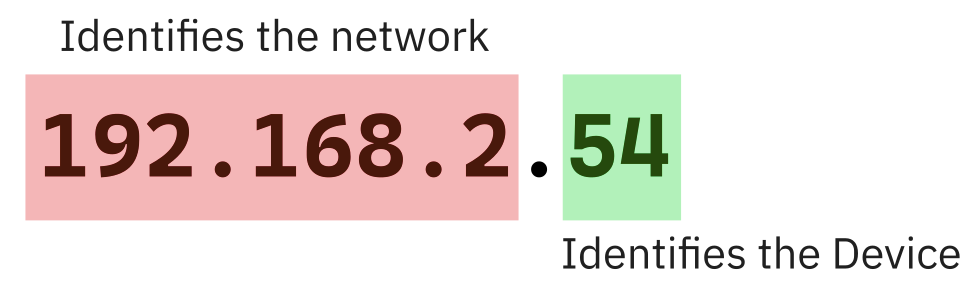
\includegraphics[width=0.7\textwidth]{ipaddr_breakdown}
    \caption{The two components of an IPv4 address}
    \label{fig:ipaddr_breakdown}
\end{figure}

Figure \ref{fig:ipaddr_breakdown} shows the two main components of IPv4 addresses; the first component determines the network itself, and the second component determines the device on the network uniquely.

\paragraph{Public IPv4 Addresses}

These IP addresses denote the location of your home router or other routers on the public internet. All web servers, like the one in our school or your personal router has a public IP address accessible by everybody\footnote{although they do not necessarily respond with data all the time}.

The only rule they must follow is that their addresses cannot be in the range of \hyperref[tab:private_ip_classes]{private IP addresses}.

% TODO: graphics?

\paragraph{Private IPv4 Addresses}

Private IP addresses are like public IP addresses, but instead of it being publicly accessible to everybody on the internet, they are only accessible to users connected to a private network, like a phone hotspot or the network created by your router. Every device on, say, your home network like your phone or your mom's work laptop have a private IP. These addresses are then mapped to public IP addresses through NATs (Network Address Translators); more details in section \ref{2:sec:nats}.

In the IPv4 address range, addresses are reserved for private networks to use, and they are:\footnote{Taken from \url{https://www.geeksforgeeks.org/private-ip-addresses-in-networking/}}

\begin{figure}[ht]
    \centering
    \begin{tabular}{ |c|c|c| }
        \hline
        \textbf{Class} & \textbf{IP Range} & \textbf{Most typically seen in} \\ \hline 
        A & {\ccmono 10.0.0.0} to {\ccmono 10.255.255.255}     & Large networks \\ \hline
        B & {\ccmono 172.16.0.0} to {\ccmono 172.31.255.255}   & Medium-sized networks \\ \hline 
        C & {\ccmono 192.168.0.0} to {\ccmono 192.168.255.255} & Small networks \\
        \hline
    \end{tabular}
    \caption{Table of private IP classes}
    \label{tab:private_ip_classes}
\end{figure}

Note that you do not need to memorize the class letters nor the exact ranges, you just need to identify them, especially the most common one, class C which is between {\ccmono 192.168.0.0} to {\ccmono 192.168.255.255}.

These private IPs belong in a local network, where devices in the same approximate geographical location are connected to a router.

\subsection{IPv4 Address Assignment}

When you connect to the school network or your home WiFi network, you need to get an IP address to \emph{identify yourself on the network}, and to allow for data transmission. Without it, no device would be able to send you data, as they won't know where you are on the network.

You may interpret it as an address to your home. A delivery driver would not be able to send you anything if you don't have an address

\subsubsection{Static IP assignment}

Static IP assignment involves your device \emph{declaring to the router} that your IP address is so and so, an address that you assign to yourself. It is set to you for an indefinite\footnote{not infinite, just an unknown amount of time} amount of time, i.e. until you choose a new address.

\textbf{Pros include:}
\begin{itemize}
    \item It is good for servers, because your location on the network does not change. Computers on the network will be able to find you easier.
    \item The connection process is much faster, as you don't have to ask for one.
    % TODO: link up static NATs
    \item You get faster upload/download speeds (only if you use a static NAT!\footnote{You will learn about NATs in a later section. Here, it means that a private address is directly mapped to the public address of your router.})
\end{itemize}

\textbf{Cons include:}
\begin{itemize}
    \item on a large private network, your location on the network is more easily identifiable, as your IP doesn't change.
    \item you cannot tell if the IP you assigned to yourself is available or not.\footnote{You can always ping the IP address to see if a device at that IP responds. If there is no response, there is no device at the IP.}
    \item it is expensive to maintain, as the device at the address must constantly be on to be available.
\end{itemize}

\subsubsection{Dynamic IP assignment}

% TODO: diagram

This method involves your device \textbf{asking the router for an IP address}. Your device communicates with a component of the router, called a \textbf{DHCP server} with the \textbf{Dynamic Host Configuration Protocol (DHCP)}, which detects which IP addresses are available, and assigns you the most optimal one.

This is by far the most common method.

\textbf{Pros include:}
\begin{itemize}
    \item On large public networks, it tends to change more often, making it more secure.
    \item It is a lot more convenient, as the device does not have to set their own IP before connecting.
\end{itemize}

\textbf{Cons include:}
\begin{itemize}
    \item If you're connected to a video call or voice call through VoIP\footnote{Basically making phone or video calls through a network and not cell towers.}, if your IP address changes, it may disconnect the call\footnote{It is not necessarily true, as your IP is not jumbled at regular intervals.}.
    \item If your device is old and does not support the DHCP protocol, you cannot use it. In short, it may not support all devices.
    \item Connection time takes longer, you must send a {\ccmono DHCPLEASE} message to the router for the IP, the router must calculate an IP, and the router must send a {\ccmono DHCPBACK} with your IP. This typically takes 5 seconds but may take up to 25 seconds.
\end{itemize}

\subsection{MAC addresses}
\label{2:sec:mac}

MAC addresses are 48 bit numbers that identify your device uniquely on any given network. They are typically represented as 3 hexadecimal numbers:

\begin{figure}[ht]
    \centering
    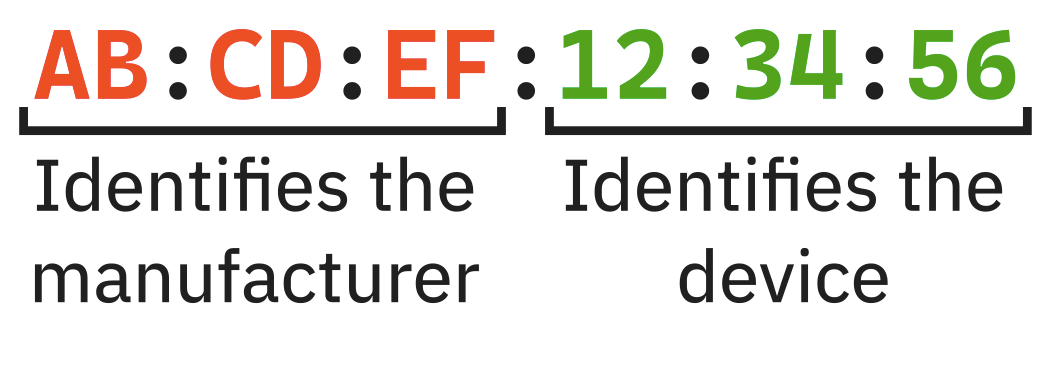
\includegraphics[width=0.7\textwidth]{macaddress_breakdown.png}
    \caption{A breakdown of the portions of a MAC address.}
    \label{fig:macaddress_breakdown}
\end{figure}

The first 3 hexadecimal bytes (2 digits) identify the maker of the device\footnote{Technically the NIC or Network Interface Card itself}, like Apple\footnote{Not necessarily, again, it identifies the maker of the NIC.}. The last 3 digits uniquely identifies the device itself.

\begin{figure}[ht]
    \centering
    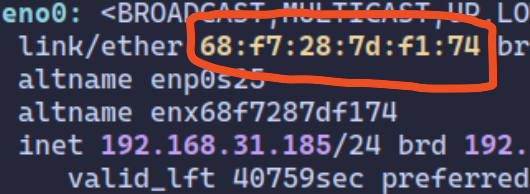
\includegraphics[width=0.7\textwidth]{macaddress.png}
    \caption{The MAC address of a computer, running Arch Linux.}
    \label{fig:macaddress}
\end{figure}

Figure \ref{fig:macaddress} shows the MAC address of one of my computers. The first 3 components identify the manufacturer, and the last 3 uniquely identifiers my device.\footnote{In this example, I have changed the default MAC address to a randomized one, so the manufacturer may be invalid if you try to look it up.}

\subsubsection{Universally Administered (UAA)}

These addresses are by far the most common; they are the addresses assigned by manufacturers and universally identify the device. They are used to ensure the unique identification of the device throughout the globe, and avoids conflicts with other MAC addresses.

\begin{itemize}
    \item These are the addresses assigned by the manufacturer stored on your NIC (see \ref{3:sec:network_hardware}).
    \item When a MAC address is mentioned, this is what one typically refers to.
    \item These uniquely identify you across multiple networks, and avoids conflicts with other MAC addresses.
\end{itemize}

\subsubsection{Locally Administered}

These addresses are a lot less common, but they have some unique properties:

\begin{itemize}
    \item They are assigned by network administrators for a particular network, not by the manufacturer.
    \item These addresses do not guarantee a unique address from router-to-router.
    \item These are only used in cases where certain MAC addresses may conflict with each other, or when a firewall needs to restrict certain devices on the network but not all of them. THese are also used in things like mainframes or cluster computers.
    \item Likewise, they can also be used to bypass a firewall.
\end{itemize}

\emph{Extra: LAA addresses also have a property where the 7th bit of the 1st byte of the MAC address is set to 1. UAA addresses have that bit set to 0.}

\subsection{Differences between IP and MAC addresses}

\begin{longtable}{|p{0.4\textwidth}|p{0.4\textwidth}|}
    \hline 
    \textbf{MAC addresses} & \textbf{IP addresses}
    \\ \hline
Identifies unique information about a device on a network & Identifies the location of something on a network
    \\ \hline
    Unique for the device on the network & Only unique if it is a public IP. Private IPs are only unique to that network, and addresses across many private IPs may be the same, as they are powered by different routers.
    \\ \hline
    48 bits & 32 bits for IPv4, or 128 bits for IPv6
    \\ \hline
    Can be locally or universally administered & Can be static or dynamic
    \\ \hline
    Assigned by the manufacturer and is baked into the NIC & Static IPs are assigned by the connecting device. Dynamic IPs are assigned by the DHCP server, usually built into the router.
    \\ \hline
\end{longtable}

\subsection{NATs (Network Address Translation)}
\label{2:sec:nats}

By now you should be familiar with the concept of private versus public IPs. Private IP addresses only exist on internal private networks, and are separate from all public IPs. How do devices on private IPs then transmit data to websites on public networks?

NATs allow private IP addresses and public IP addresses to be tempoarily linked together to create a channel whereby data can flow. These are typically in your home router to map devices connected to it to the router's public IP address.

\begin{figure}[h]
    \centering
    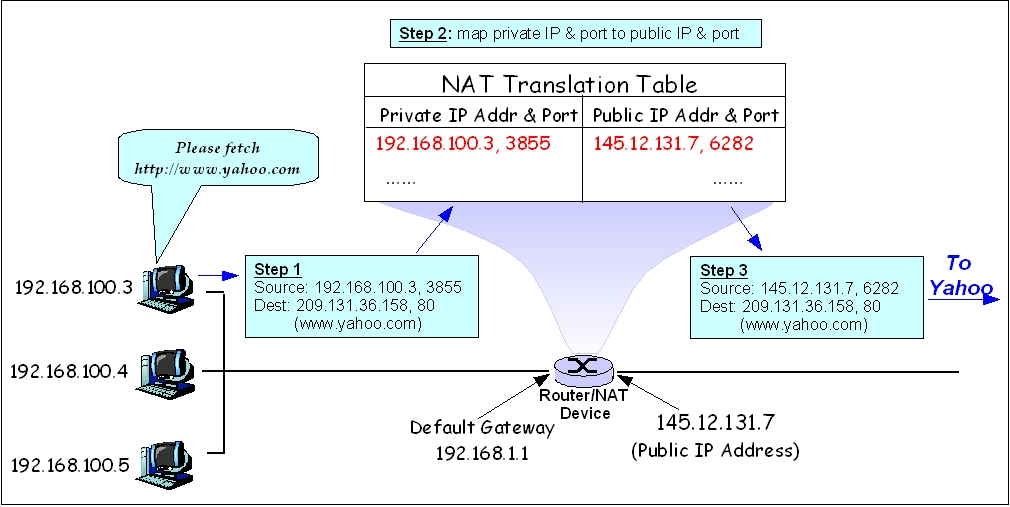
\includegraphics[width=0.7\textwidth]{nat.jpg}
    \caption{A diagram explaining how network addresses are mapped to public IPs through the NAT. Taken from Wikipedia.}
    \label{fig:nat}
\end{figure}

Figure \ref{fig:nat} depicts home computers on a network that requests to visit a website, like Yahoo\footnote{One could presume that this image is quite old}. A lookup table is established in the router, where the IP the computer has is associated with the IP of yahoo. This then allows the devices to begin packet switching through this device\footnote{Do not worry about the port; this allows 65535 channels of data to be open on one IP address, as one single IP is quite limiting.}.


\end{document}
